
\begin{figure}
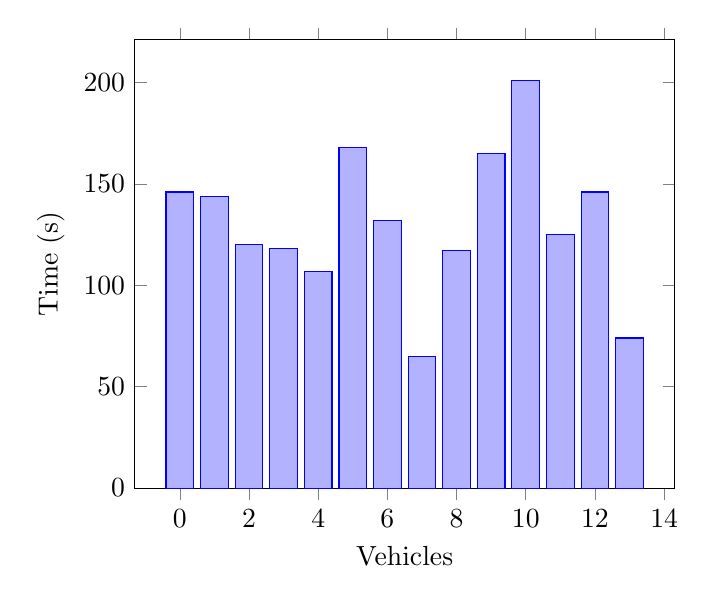
\begin{tikzpicture}
\begin{axis}[
legend style={anchor=west},
xlabel=Vehicles,
ylabel=Time (s),
ymin=0,
ybar,
]
\addplot coordinates {
(0, 146)
(1, 144)
(2, 120)
(3, 118)
(4, 107)
(5, 168)
(6, 132)
(7, 65)
(8, 117)
(9, 165)
(10, 201)
(11, 125)
(12, 146)
(13, 74)
};

\end{axis}
\end{tikzpicture}
\label{tik:100:6_O, 6_O.-30, 7_S, 7_S.-25, 11_S, 11_S.-50, 13_S, 15_N, 17_S, 17_S.-60, 18_S}
\caption{100 percent diving with GSC on route $6_O, 6_O.-30, 7_S, 7_S.-25, 11_S, 11_S.-50, 13_S, 15_N, 17_S, 17_S.-60, 18_S$}
\end{figure}
